\documentclass[12pt,a4paper]{article}

\usepackage[utf8]{inputenc}
\usepackage[T1]{fontenc}
\usepackage[spanish]{babel}
\usepackage{geometry}
\usepackage{amsmath,amssymb}
\usepackage{booktabs}
\usepackage{array}
\usepackage{graphicx}
\usepackage{xcolor}
\usepackage{listings}
\usepackage{hyperref}
\usepackage{fancyhdr}
\usepackage{titlesec}
\usepackage{enumitem}
\usepackage{float}
\usepackage{multirow}
\usepackage{colortbl}

\geometry{margin=2.5cm, top=3cm, bottom=3cm}

\definecolor{unsa-blue}{RGB}{0,56,147}
\definecolor{code-bg}{RGB}{248,248,248}
\definecolor{code-kw}{RGB}{0,0,180}
\definecolor{code-str}{RGB}{163,21,21}
\definecolor{code-cm}{RGB}{0,128,0}
\definecolor{verde}{RGB}{39,174,96}
\definecolor{rojo}{RGB}{192,57,43}
\definecolor{cons100}{RGB}{212,237,218}
\definecolor{compareA}{RGB}{240,248,255}
\definecolor{compareB}{RGB}{238,255,238}
\definecolor{compareC}{RGB}{255,248,225}

\lstdefinestyle{output}{
    backgroundcolor=\color{gray!8},
    basicstyle=\ttfamily\small,
    frame=single, framerule=0.4pt, rulecolor=\color{gray!40},
    breaklines=true, numbers=none, xleftmargin=0.5em, captionpos=b,
}

\pagestyle{fancy}
\fancyhf{}
\fancyhead[L]{\small\textcolor{unsa-blue}{\textbf{Computación Gráfica — Lab 09}}}
\fancyhead[R]{\small\textcolor{unsa-blue}{UNSA-EPCC 2026A}}
\fancyfoot[C]{\small\thepage}
\renewcommand{\headrulewidth}{0.4pt}

\titleformat{\section}{\large\bfseries\color{unsa-blue}}{}{0em}{}[\titlerule]
\titleformat{\subsection}{\normalsize\bfseries\color{unsa-blue!80}}{}{0em}{}
\titleformat{\subsubsection}{\normalsize\itshape}{}{0em}{}

\hypersetup{colorlinks=true,linkcolor=unsa-blue,urlcolor=unsa-blue}

\begin{document}

% ── Portada ──────────────────────────────────────────────────────────────────
\begin{titlepage}
\centering\vspace*{1cm}
{\Large\bfseries\color{unsa-blue}
  Universidad Nacional de San Agustín de Arequipa\\[0.3em]
  Escuela Profesional de Ciencia de la Computación}\\[2em]
\rule{\linewidth}{1.5pt}\\[0.8em]
{\LARGE\bfseries Laboratorio 09}\\[0.4em]
{\large Escenas 3D, Materiales, Iluminación y Texturas}\\[0.3em]
{\large\itshape Computación Gráfica — 2026A}\\[0.4em]
\rule{\linewidth}{1.5pt}\\[2em]
\begin{tabular}{ll}
  \textbf{Curso}    & Computación Gráfica \\[0.3em]
  \textbf{Docente}  & MG. R. Jesús Cárdenas Talavera \\[0.3em]
  \textbf{Lenguaje} & C++ / OpenGL / GLFW / ImGui \\[0.3em]
  \textbf{Alumno}   & Percy Maldonado Quispe \\[0.3em]
  \textbf{Fecha}    & Junio 2026 \\
\end{tabular}
\vfill
\end{titlepage}

\tableofcontents\newpage

% ══════════════════════════════════════════════════════════════════════════════
\section{Introducción}
% ══════════════════════════════════════════════════════════════════════════════

En este laboratorio se construyó una escena 3D compuesta por un terreno, una
casa y un árbol, y luego se representó de tres maneras distintas para comparar
visual y técnicamente el efecto de los materiales, la iluminación y las
texturas.

La idea principal del trabajo no fue solo cumplir con el modelo 3D, sino
\textbf{comparar} tres enfoques de representación sobre la misma geometría:

\begin{itemize}[noitemsep]
  \item \textbf{Escena 1:} solo materiales.
  \item \textbf{Escena 2:} texturas procedurales generadas en código.
  \item \textbf{Escena 3:} texturas reales cargadas desde archivos de imagen.
\end{itemize}

Esta comparación permite ver con claridad cómo cambia la apariencia visual sin
alterar la estructura de la escena.

% ══════════════════════════════════════════════════════════════════════════════
\section{Objetivos}
% ══════════════════════════════════════════════════════════════════════════════

\subsection{Objetivo general}

Comprender la construcción de escenas tridimensionales en OpenGL mediante el
uso de primitivas geométricas, materiales, iluminación y texturas.

\subsection{Objetivos específicos}

\begin{enumerate}[noitemsep]
  \item Construir una escena con terreno, casa y árbol.
  \item Definir materiales diferentes para cada objeto.
  \item Configurar iluminación direccional y puntual.
  \item Comparar texturas procedurales con texturas cargadas desde imágenes.
  \item Organizar tres escenas equivalentes para realizar una comparación
        visual directa.
\end{enumerate}

% ══════════════════════════════════════════════════════════════════════════════
\section{Descripción de la escena 3D}
% ══════════════════════════════════════════════════════════════════════════════

La escena base es la misma en las tres versiones:

\begin{itemize}[noitemsep]
  \item \textbf{Terreno:} plano de 40\,x\,40 unidades centrado en el origen.
  \item \textbf{Casa:} ubicada sobre el terreno, con paredes y techo diferenciados.
  \item \textbf{Árbol:} tronco cilíndrico y copa esférica, cercano a la casa.
\end{itemize}

La organización espacial fue diseñada para que el usuario pueda comparar los
cambios visuales entre escenas sin cambiar la geometría.

\subsection{Estructura general de la implementación}

El proyecto se organizó en varios archivos para mantener el código limpio:

\begin{center}
\begin{tabular}{ll}
\toprule
\textbf{Archivo} & \textbf{Responsabilidad} \\
\midrule
\texttt{main.cpp} & Ventana, menú, cámara, selección de escena \\
\texttt{Scene.h} & Clase base de escena \\
\texttt{SceneMaterials.h} & Escena 1: materiales \\
\texttt{SceneProcedural.h} & Escena 2: texturas procedurales \\
\texttt{SceneTextured.h} & Escena 3: texturas reales \\
\texttt{Geometry.h} & Terreno, casa, árbol y primitivas \\
\texttt{Material.h} & Definición y aplicación de materiales \\
\texttt{TextureManager.h} & Carga y generación de texturas \\
\bottomrule
\end{tabular}
\end{center}

% ══════════════════════════════════════════════════════════════════════════════
\section{Materiales e iluminación}
% ══════════════════════════════════════════════════════════════════════════════

\subsection{Materiales}

En la escena de materiales, cada parte del modelo tiene propiedades propias:
componente ambiental, difusa, especular y brillo. Esto permite que el mismo
modelo se vea distinto según el objeto.

\begin{itemize}[noitemsep]
  \item Terreno: color verde y brillo bajo.
  \item Paredes: rojo mate.
  \item Techo: rojo/plomo con un brillo más visible.
  \item Tronco: marrón con componente especular moderada.
  \item Copa: verde más oscuro y menos brillante.
\end{itemize}

La idea es que el material sea responsable del aspecto visual base antes de
aplicar textura.

\subsection{Iluminación}

El proyecto utiliza el sistema clásico de iluminación de OpenGL:

\begin{itemize}[noitemsep]
  \item luz ambiental,
  \item luz difusa,
  \item luz especular.
\end{itemize}

Se probó una \textbf{luz direccional} y una \textbf{luz puntual} para observar
cómo cambian las sombras y los reflejos. La luz direccional simula una fuente
lejana y uniforme, mientras que la puntual genera una iluminación más localizada
con atenuación espacial.

\subsection{Estado gráfico activado}

Además de la iluminación, se activaron estados de render importantes para mejorar
la calidad de la escena:

\begin{lstlisting}[style=output]
glShadeModel(GL_SMOOTH);
glEnable(GL_CULL_FACE);
glEnable(GL_DEPTH_TEST);
glDepthFunc(GL_LEQUAL);
glHint(GL_PERSPECTIVE_CORRECTION_HINT, GL_NICEST);
\end{lstlisting}

% ══════════════════════════════════════════════════════════════════════════════
\section{Texturizado}
% ══════════════════════════════════════════════════════════════════════════════

\subsection{Escena 2: texturas procedurales}

En esta versión, las texturas se generan por código. Esto tiene dos ventajas:

\begin{itemize}[noitemsep]
  \item no depende de archivos externos,
  \item permite controlar el patrón visual con precisión.
\end{itemize}

Por ejemplo, pueden generarse patrones de césped, ladrillo, tejas, madera y
hojas sin usar imágenes reales.

\subsection{Escena 3: texturas reales}

En esta versión se cargan imágenes externas con una librería de lectura de
texturas, como \texttt{stb\_image.h}. Cada archivo de imagen se
convierte a una textura OpenGL y se asigna a cada objeto de la escena.

Texturas usadas:

\begin{itemize}[noitemsep]
  \item césped para el terreno,
  \item ladrillo para las paredes,
  \item tejas para el techo,
  \item madera para el tronco,
  \item hojas para la copa.
\end{itemize}

\subsection{Coordenadas de textura}

Para evitar deformaciones visibles, se ajustaron las coordenadas UV según la
superficie de cada objeto. Esto es especialmente importante en el terreno y en
las caras del techo, donde una mala parametrización puede estirar o repetir la
imagen de forma incorrecta.

% ══════════════════════════════════════════════════════════════════════════════
\section{Comparación de las tres escenas}
% ══════════════════════════════════════════════════════════════════════════════

Esta es la parte más importante del informe, porque resume por qué conviene
mostrar las tres versiones de la misma escena.

\begin{center}
\begin{tabular}{p{2.5cm} p{4.2cm} p{4.2cm} p{4.2cm}}
\toprule
\textbf{Aspecto} & \textbf{Escena 1: Materiales} & \textbf{Escena 2: Procedurales} & \textbf{Escena 3: Reales} \\
\midrule
Apariencia & Depende solo de los parámetros del material y la luz. & Mejora la apariencia con patrones generados en código. & Mayor realismo por uso de imágenes reales. \\
Dependencia externa & No requiere archivos de imagen. & No requiere archivos de imagen. & Sí requiere archivos \texttt{.png/.jpg}. \\
Control visual & Más simple y técnico. & Flexible y útil para pruebas. & Más realista y cercano a producción. \\
Realismo & Bajo/medio. & Medio. & Alto. \\
Costo de implementación & Bajo. & Medio. & Medio/alto por carga y coordenadas UV. \\
\bottomrule
\end{tabular}
\end{center}

\subsection{Observación visual}

La comparación permite ver que:

\begin{itemize}
  \item los \textbf{materiales} controlan la respuesta a la luz,
  \item las \textbf{texturas procedurales} agregan detalle sin archivos externos,
  \item las \textbf{texturas reales} aportan mayor fidelidad visual.
\end{itemize}

Por eso, sí tiene sentido presentar las tres escenas: no es redundante, sino que
sirve para mostrar la evolución desde una representación básica hasta una más
realista.

% ══════════════════════════════════════════════════════════════════════════════
\section{Resultados}
% ══════════════════════════════════════════════════════════════════════════════

Se obtuvo una aplicación interactiva donde el usuario puede:

\begin{itemize}[noitemsep]
  \item cambiar entre las tres escenas con las teclas 1, 2 y 3,
  \item alternar luz direccional y puntual con la tecla L,
  \item rotar la cámara con el mouse,
  \item hacer zoom con la rueda del mouse.
\end{itemize}

\subsection{Capturas}

\begin{figure}[H]
\centering
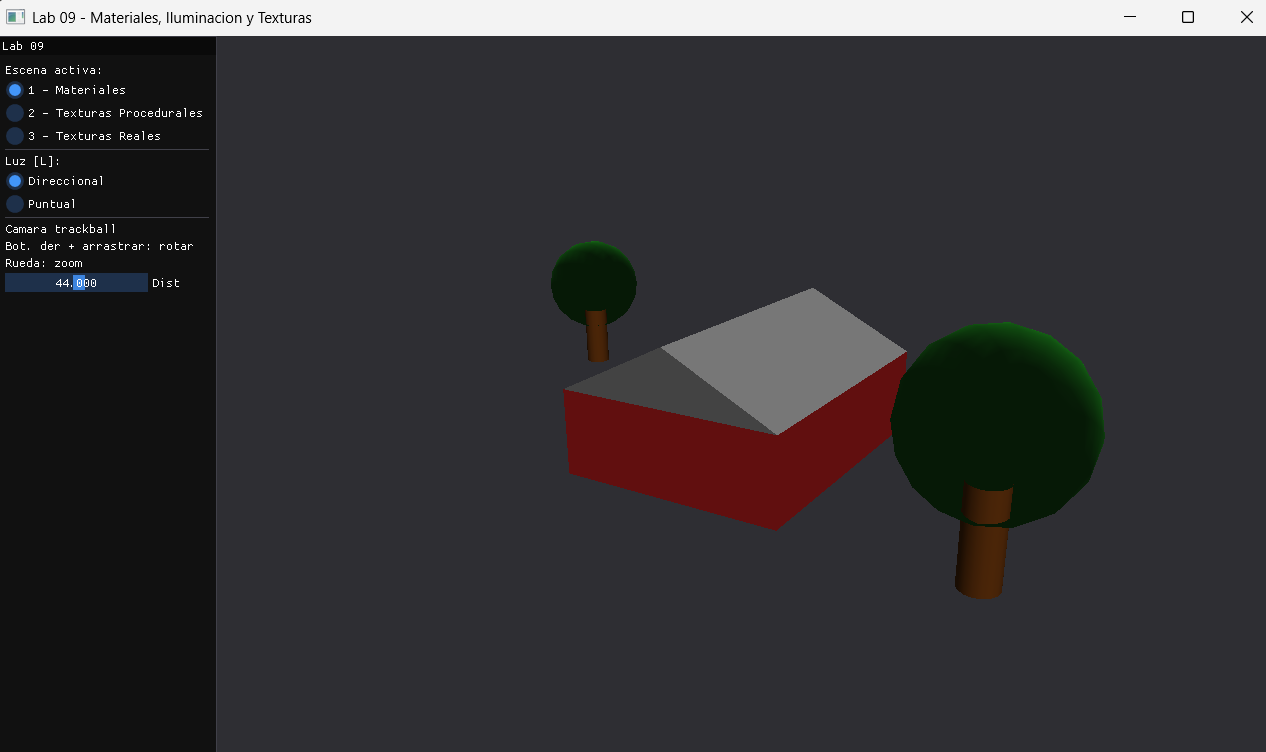
\includegraphics[width=0.92\textwidth]{screenshots/scene1_materials.png}
\caption{Escena 1: solo materiales.}
\end{figure}

\begin{figure}[H]
\centering
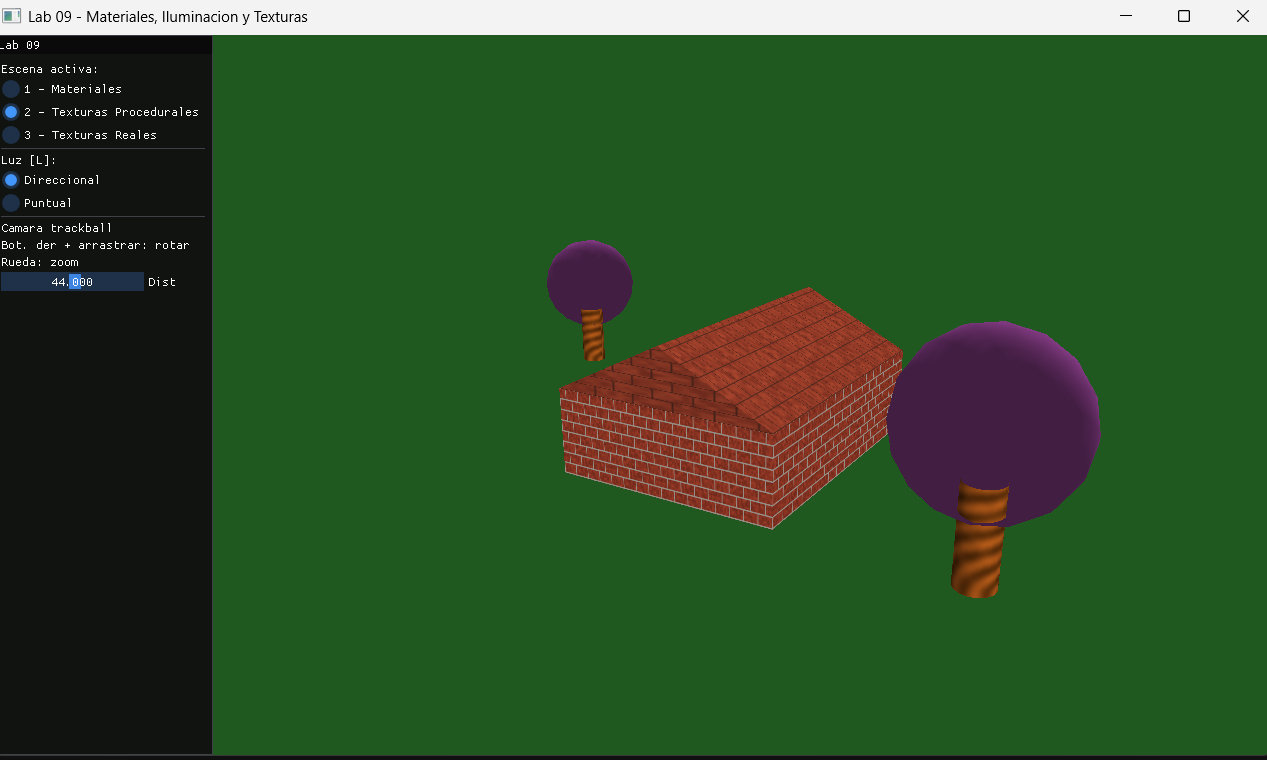
\includegraphics[width=0.92\textwidth]{screenshots/scene2_procedural.png}
\caption{Escena 2: texturas procedurales.}
\end{figure}

\begin{figure}[H]
\centering
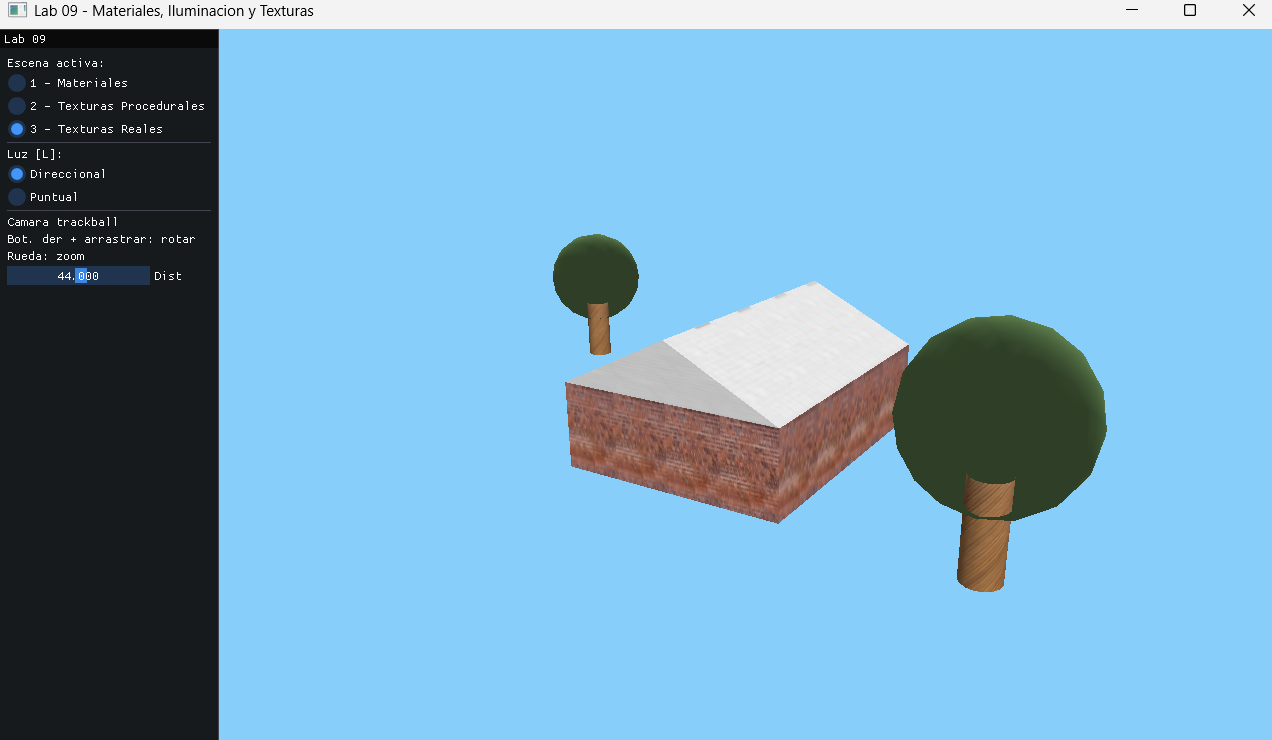
\includegraphics[width=0.92\textwidth]{screenshots/scene3_textured.png}
\caption{Escena 3: texturas reales.}
\end{figure}

\begin{figure}[H]
\centering
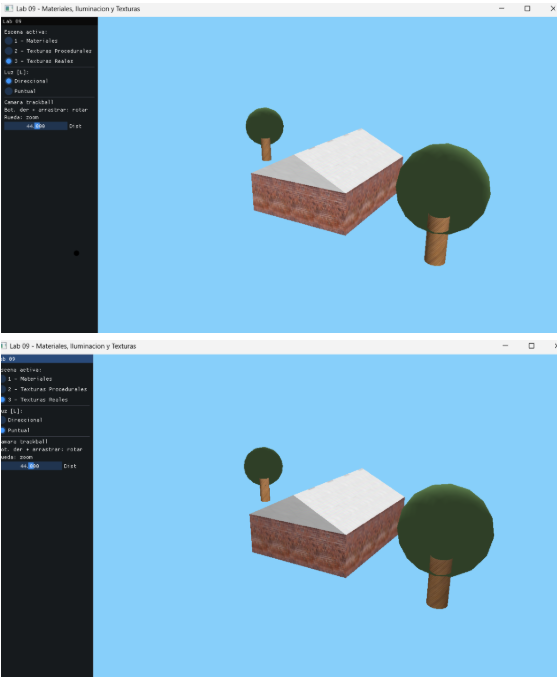
\includegraphics[width=0.92\textwidth]{screenshots/lighting_compare.png}
\caption{Comparación entre luz direccional y puntual.}
\end{figure}

% ══════════════════════════════════════════════════════════════════════════════
\section{Conclusiones}
% ══════════════════════════════════════════════════════════════════════════════

\begin{enumerate}
  \item La misma geometría puede verse muy distinta según el uso de
        materiales, texturas procedurales o texturas reales.
  \item Las texturas procedurales son una buena alternativa cuando se desea
        independencia de archivos externos.
  \item Las texturas reales ofrecen un mayor realismo visual, aunque dependen
        de imágenes adicionales y de una correcta configuración UV.
  \item La iluminación direccional y puntual produce efectos diferentes que
        ayudan a entender mejor el modelo de iluminación de OpenGL.
  \item La comparación entre las tres escenas hace que el laboratorio sea más
        claro y completo que mostrar solo una versión única.
\end{enumerate}

% ══════════════════════════════════════════════════════════════════════════════
\section*{Referencias}
\addcontentsline{toc}{section}{Referencias}
% ══════════════════════════════════════════════════════════════════════════════

\begin{itemize}[noitemsep]
  \item OpenGL Architecture Review Board. \textit{OpenGL Programming Guide}.
  \item LearnOpenGL. \url{https://learnopengl.com/}
  \item stb image. \url{https://github.com/nothings/stb}
  \item Apuntes de clase de Computación Gráfica, UNSA-EPCC.
\end{itemize}

\end{document}

